%%%%%%%%%%%%%%%%%%%%%%%%%%%%%%%%%%%%

\section{5.3. Diferença de duas médias}

%%%%%%%%%%%%%%%%%%%%%%%%%%%%%%%%%%%%

\begin{frame}
\frametitle{Diamantes}

\begin{itemize}
\justifying
\item Pesos de diamantes são medidos em quilates. 
\justifying
\item 1 quilate = 100 pontos, 0,99 quilates = 99 pontos, etc.
\justifying
\item A diferença entre o tamanho de um diamante de 0,99 quilates e um diamante de 1 quilate é indetectável a olho nu, mas o preço de um diamante de 1 quilate tende a ser maior do que o preço de um diamante de 0,99 quilates?
\justifying
\item Vamos testar para ver se existe uma diferença entre os preços médios de diamantes de 0,99 e 1 quilates.
\justifying
\item Para podermos comparar unidades equivalentes, dividimos os preços de 0,99 quilates em 99 e de 1 quilate em 100, e comparamos os preços médios em pontos.

\end{itemize}

\hfill 
\includegraphics[width=0.2\textwidth]{5-3_diff_two_mean/diamond.png}

\end{frame}

%%%%%%%%%%%%%%%%%%%%%%%%%%%%%%%%%%%

\begin{frame}[fragile]
\frametitle{Dados}

\begin{center}
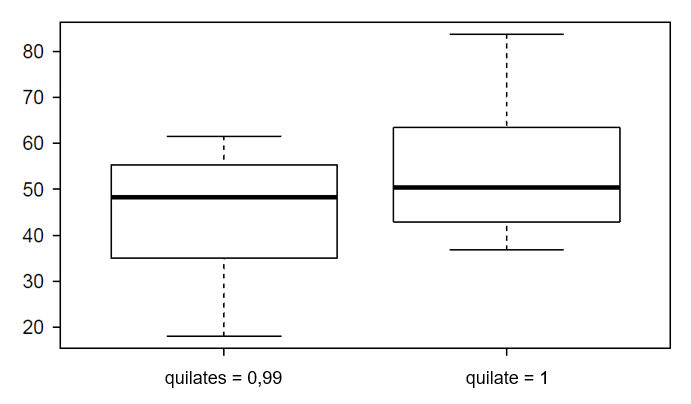
\includegraphics[width=0.6\textwidth]{5-3_diff_two_mean/diamondBox.png}
\end{center}

{\small
\begin{center}
\begin{tabular}{l | c | c}
		& {\footnotesize \hl{0.99 quilate}} &  {\footnotesize \hl{1 quilate}}  \\
		& pt99	& pt100 \\
\hline
$\bar{x}$	& 44.50		& 53.43 \\
$s$		& 13.32		& 12.22 \\
$n$		& 23			& 30
\end{tabular}
\end{center}
}

\vfill

\rule{2.5cm}{0.25pt} \\
\justifying
{\tiny Estes dados são uma amostra aleatória do conjunto de dados \texttt {diamonds} no pacote do R \texttt {ggplot2}.}

\end{frame}

%%%%%%%%%%%%%%%%%%%%%%%%%%%%%%%%%%%

\begin{frame}
\frametitle{Estimativa de parâmetro e ponto}

\begin{itemize}
\justifying
\item \hl{Parâmetro de interesse:} Diferença média entre os preços em pontos de \orange{todos} os diamantes de 0,99 quilates e de 1 quilate.
\[ \mu_{pt99} - \mu_{pt100} \]

$\:$ \\

\pause
\justifying
\item \hl{Estimativa pontual:} Diferença média entre os preços em pontos da \orange{amostra} de diamantes de 0,99 quilates e 1 quilate.
\[ \bar{x}_{pt99} - \bar{x}_{pt100} \]

\end{itemize}

\end{frame}

%%%%%%%%%%%%%%%%%%%%%%%%%%%%%%%%%%%

\begin{frame}
\frametitle{Hipótese}
\justifying
\pq{Qual das alternativas a seguir é o conjunto correto de hipóteses para testar se o preço médio dos diamantes de 1 quilate ($ _{pt100} $) é maior que o preço médio dos diamantes de 0,99 quilates ($_{pt99}$)?}

\begin{enumerate}[(a)]

\item  \mathhl{H_0:} $\mu_{pt99} = \mu_{pt100}$ \\
\mathhl{H_A:} $\mu_{pt99} \ne \mu_{pt100}$

\item  \mathhl{H_0:} $\mu_{pt99} = \mu_{pt100}$ \\
\mathhl{H_A:} $\mu_{pt99} > \mu_{pt100}$

\solnMult{  \mathhl{H_0:} $\mu_{pt99} = \mu_{pt100}$ \\
\mathhl{H_A:} $\mu_{pt99} < \mu_{pt100}$ }

\item  \mathhl{H_0:} $\bar{x}_{pt99} = \bar{x}_{pt100}$ \\
\mathhl{H_A:} $\bar{x}_{pt99} < \bar{x}_{pt100}$

\end{enumerate}

\end{frame}

%%%%%%%%%%%%%%%%%%%%%%%%%%%%%%%%%%%

\begin{frame}
\frametitle{Condições}
\justifying
\pq{Qual dos seguintes itens \underline{não} precisa ser satisfeito para conduzir este teste de hipótese usando métodos teóricos?}

\begin{enumerate}[(a)]
\justifying
\item O preço do ponto de um diamante de 0,99 quilates na amostra deve ser independente do outro, e o preço em pontos de um diamante de 1 quilate deve ser independente do outro.
\justifying
\item Os preços pontuais de 0,99 quilates e 1 quilate de diamantes na amostra devem ser independentes.
\justifying
\item Distribuições de preços pontuais de 0,99 e 1 quilate de diamantes não devem ser extremamente assimétrico.
\justifying
\solnMult{Ambos os tamanhos de amostra devem ser pelo menos 30.}

\end{enumerate}

\end{frame}

%%%%%%%%%%%%%%%%%%%%%%%%%%%%%%%%%%%%

\subsection{Distribuição amostral para a diferença de duas médias}

%%%%%%%%%%%%%%%%%%%%%%%%%%%%%%%%%%%%

\begin{frame}
\frametitle{Estatística de teste}
\justifying
\formula{Teste estatístico para inferência sobre a diferença de duas médias amostrais pequenas}
\justifying
{A estatística de teste para inferência sobre a diferença de duas médias onde $\sigma_1$ e $\sigma_2$ são desconhecidos é a estatística $T$.
\vspace{0.3 cm}
\[ T_{df} = \frac{\text{estimativa pontual} - \text{valor da hipótese nula}}{SE} \]
onde 
\[ SE = \sqrt{ \frac{s_1^2}{n_1} + \frac{s_2^2}{n_2} } \qquad \text{ e } \qquad df = min(n_1 - 1, n_2 - 1) \]
}\justifying
\justifying
\Note{O cálculo do $df$ é realmente muito mais complicado. Para simplificar, usaremos a fórmula acima para \underline{estimar} o verdadeiro $df$ ao conduzir a análise à mão.}

\end{frame}

%%%%%%%%%%%%%%%%%%%%%%%%%%%%%%%%%%%%

\subsection{Teste de hipóteses para a diferença de duas médias}

%%%%%%%%%%%%%%%%%%%%%%%%%%%%%%%%%%%%

\begin{frame}
\frametitle{Estatística de teste (cont.)}

{\small
\begin{center}
\begin{tabular}{l | c | c}
		& {\footnotesize \hl{0.99 quilate}} &  {\footnotesize \hl{1 quilate}}  \\
		& pt99	& pt100 \\
\hline
$\bar{x}$	& 44.50		& 53.43 \\
$s$		& 13.32		& 12.22 \\
$n$		& 23			& 30
\end{tabular}
\end{center}
}

\hl{Neste contexto...}

\pause

{\small
\begin{eqnarray*}
T &=& \frac{\text{estimativa pontual} - \text{valor da hipótese nula} }{SE} \\
\pause
&=& \frac{(44.50 - 53.43) - 0}{ \sqrt{\frac{13.32^2}{23} + \frac{12.22^2}{30} }} \\
\pause
&=& \frac{-8.93}{3.56} \\
\pause
&=& -2.508
\end{eqnarray*}
}

\end{frame}

%%%%%%%%%%%%%%%%%%%%%%%%%%%%%%%%%%%%

\begin{frame}
\frametitle{Estatística de teste (cont.)}
\justifying
\pq{Qual dos seguintes é o $df$ correto para este teste de hipótese?}

\twocol{0.3}{0.7}
{
\begin{enumerate}[(a)]
\solnMult{ 22 }
\item 23
\item 30
\item 29
\item 52
\end{enumerate}
}
{
\soln{\only<2>{
\orange{$\rightarrow df = min(n_{pt99} - 1, n_{pt100} - 1)$ \\
$= min(23 - 1, 30 - 1)$ \\
$= min(22,29) = 22$} \\
\vspace{1cm}
}}}

\end{frame}

%%%%%%%%%%%%%%%%%%%%%%%%%%%%%%%%%%%%

\begin{frame}
\frametitle{valor-p}
\justifying
\pq{Qual dos seguintes é o valor p correto para este teste de hipótese?}

\[ T = -2.508 \qquad \only<1-2 | handout:0>{df = 22} \] 

\twocol{0.42}{0.58}
{
\begin{enumerate}[(a)]
\item entre 0.005 e 0.01
\solnMult{entre 0.01 e 0.025}
\item entre 0.02 e 0.05
\item entre 0.01 e 0.02
\end{enumerate}
}
{
\only<1>{
{
\scalefont{0.47}
\begin{tabular}{r | r r  r r r}
\hline
uma cauda & \hspace{1.5mm}  0.100 & \hspace{1.5mm} 0.050 & \hspace{1.5mm} {0.025} & \hspace{1.5mm} {0.010} & \hspace{1.5mm} 0.005  \\
duas caudas & 0.200 & 0.100 & 0.050 & 0.020 & 0.010 \\
\hline
df \hfill 21  &  {  1.32} & {  1.72} & {  2.08} & {  2.52} & {  2.83}  \\ 
22  &  {  1.32} & {  1.72} & {  2.07} & {  2.51} & {  2.82}  \\ 
23  &  {  1.32} & {  1.71} & {  2.07} & {  2.50} & {  2.81}  \\ 
24  &  {  1.32} & {  1.71} & {  2.06} & {  2.49} & {  2.80}  \\ 
25  &  {  1.32} & {  1.71} & {  2.06} & {  2.49} & {  2.79}  \\ 
\hline
\end{tabular}
}
}

\only<2|handout:0>{
{\scalefont{0.47}
\begin{tabular}{r | r r  >{\columncolor[gray]{.6}[.5\tabcolsep]}r  >{\columncolor[gray]{.6}[.5\tabcolsep]}r r}
\hline
uma cauda & \hspace{1.5mm}  0.100 & \hspace{1.5mm} 0.050 & \hspace{1.5mm} \orange{0.025} & \hspace{1.5mm} \orange{0.010} & \hspace{1.5mm} 0.005  \\
duas caudas & 0.200 & 0.100 & 0.050 & 0.020 & 0.010 \\
\hline
df \hfill 21  &  {  1.32} & {  1.72} & {  2.08} & {  2.52} & {  2.83}  \\ 
  \rowcolor[gray]{.6}
22  &  {  1.32} & {  1.72} & \orange{  2.07} & \orange{  2.51} & {  2.82}  \\ 
23  &  {  1.32} & {  1.71} & {  2.07} & {  2.50} & {  2.81}  \\ 
24  &  {  1.32} & {  1.71} & {  2.06} & {  2.49} & {  2.80}  \\ 
25  &  {  1.32} & {  1.71} & {  2.06} & {  2.49} & {  2.79}  \\ 
\hline
\end{tabular}
}
}}

\end{frame}

%%%%%%%%%%%%%%%%%%%%%%%%%%%%%%%%%%%%

\begin{frame}
\frametitle{Síntese}
\justifying
\dq{Qual é a conclusão do teste de hipóteses? Como essa conclusão mudaria seu comportamento se você comprasse diamantes?}


\soln{\only<2>{
\begin{itemize}
\justifying
\item O valor p é pequeno, portanto, rejeite $H_0$. Os dados fornecem evidências convincentes para sugerir que o preço em pontos de 0,99 quilates é menor do que o preço em pontos de 1 quilate de diamantes.
\justifying
\item Talvez compre um diamante de 0,99 quilates? É quase um quilate, mas é significativamente mais barato.
\end{itemize}
}}

\end{frame}

%%%%%%%%%%%%%%%%%%%%%%%%%%%%%%%%%%%%

\subsection{Intervalos de confiança para a diferença de duas médias}

%%%%%%%%%%%%%%%%%%%%%%%%%%%%%%%%%%%%

\begin{frame}
\frametitle{Nível de confiança equivalente}
\justifying
\pq{Qual é o nível de confiança equivalente para um teste de hipótese unilateral para $\alpha = 0.05$?}


\twocol{0.3}{0.7}{
\begin{enumerate}[(a)]

\solnMult{90\%}

\item 92.5\%

\item 95\%

\item 97.5\%

\end{enumerate}
}
{
\soln{\only<2>{
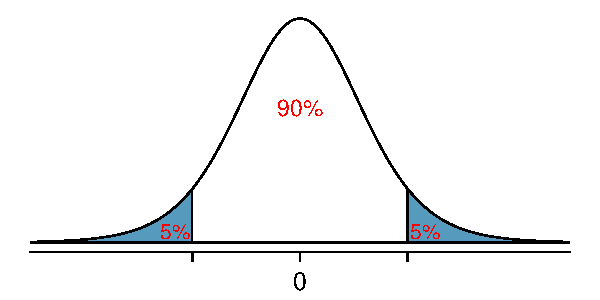
\includegraphics[width=\textwidth]{5-3_diff_two_mean/middle90.pdf}
}}
}

\end{frame}

%%%%%%%%%%%%%%%%%%%%%%%%%%%%%%%%%%%%

\begin{frame}
\frametitle{Valor crítico}
\justifying
\pq{Qual é o $ t ^ \star $ apropriado para um intervalo de confiança para a diferença média entre os preços pontuais de 0,99 e 1 quilate de diamantes?}

\begin{enumerate}[(a)]
\item 1.32
\solnMult{1.72}
\item 2.07
\item 2.82
\end{enumerate}

\only<1>{
{\small
\begin{center}
\begin{tabular}{r | r r r r r}
\hline
uma cauda & \hspace{1.5mm}  0.100 & \hspace{1.5mm} {0.050} & \hspace{1.5mm} {0.025} & \hspace{1.5mm} {0.010} & \hspace{1.5mm} 0.005  \\
duas caudas & 0.200 & 0.100 & 0.050 & 0.020 & 0.010 \\
\hline
df \hfill 21  &  {  1.32} & {  1.72} & {  2.08} & {  2.52} & {  2.83}  \\ 
22  &  {  1.32} & {  1.72} & {  2.07} & {  2.51} & {  2.82}  \\ 
23  &  {  1.32} & {  1.71} & {  2.07} & {  2.50} & {  2.81}  \\ 
24  &  {  1.32} & {  1.71} & {  2.06} & {  2.49} & {  2.80}  \\ 
25  &  {  1.32} & {  1.71} & {  2.06} & {  2.49} & {  2.79}  \\ 
\end{tabular}
\end{center}
}}

\only<2|handout:0>{
\begin{center}
{\small
\begin{tabular}{r | r >{\columncolor[gray]{.6}[.5\tabcolsep]}r r  r r}
\hline
uma cauda & \hspace{1.5mm}  0.100 & \hspace{1.5mm} {0.050} & \hspace{1.5mm} {0.025} & \hspace{1.5mm} {0.010} & \hspace{1.5mm} 0.005  \\
duas caudas & 0.200 & \orange{0.100} & 0.050 & 0.020 & 0.010 \\
\hline
df \hfill 21  &  {  1.32} & {  1.72} & {  2.08} & {  2.52} & {  2.83}  \\ 
  \rowcolor[gray]{.6}
22  &  {  1.32} & \orange{  1.72} & {  2.07} & {  2.51} & {  2.82}  \\ 
23  &  {  1.32} & {  1.71} & {  2.07} & {  2.50} & {  2.81}  \\ 
24  &  {  1.32} & {  1.71} & {  2.06} & {  2.49} & {  2.80}  \\ 
25  &  {  1.32} & {  1.71} & {  2.06} & {  2.49} & {  2.79}  \\ 
\hline
\end{tabular}
}
\end{center}
}


\end{frame}

%%%%%%%%%%%%%%%%%%%%%%%%%%%%%%%%%%%%

\begin{frame}
\frametitle{Intervalo de confiança}
\justifying
\dq{Calcule o intervalo e interprete-o no contexto.}

\pause

\soln{
\[ \text{estimativa pontual} \pm ME \]
\pause
\begin{eqnarray*}
(\bar{x}_{pt99} - \bar{x}_{pt1}) \pm t^\star_{df} \times SE &=& (44.50 - 53.43) \pm 1.72 \times 3.56 \\
\pause
&=& -8.93 \pm  6.12 \\
\pause
&=& (-15.05, -2.81)
\end{eqnarray*}
\pause
\justifying
Temos 90\% de confiança de que o preço médio de um diamante de 0,99 quilates é \$ 15,05 a \$ 2,81 abaixo do preço médio de um diamante de 1 quilate.
}

\end{frame}

%%%%%%%%%%%%%%%%%%%%%%%%%%%%%%%%%%%%

\subsection{Recap}

%%%%%%%%%%%%%%%%%%%%%%%%%%%%%%%%%%%%

\begin{frame}
\frametitle{Recapitulação: Inferência usando diferença de duas médias amostrais pequenas}
\small
\begin{itemize}
\justifying
\item Se $ \sigma_1 $ ou $ \sigma_2 $ for desconhecido, a diferença entre a amostra segue uma distribuição $t$ com $SE = \sqrt{ \frac{s_1^2}{n_1} + \frac{s_2^2}{n_1} }$.

\pause
\justifying
\item Condições: 
\begin{itemize}
\justifying
\item independência dentro dos grupos (frequentemente verificada por uma amostra aleatória, e se amostragem sem reposição, $ n <$ 10 \% da população) e entre grupos.
\justifying
\item nenhum desvio extremo em nenhum dos grupos.
\end{itemize}

\pause
\justifying
\item Teste de hipóteses: 
\[ T_{df} = \frac{\text{estimativa pontual} - \text{valor da hipótese nula}}{SE}\\\text{onde }df = min(n_1 - 1, n_2 - 1) \]

\pause
\justifying
\item Intervalo de confiança:
\[ \text{estimativa pontual} \pm t_{df}^\star \times SE \]

\end{itemize}

\end{frame}

%%%%%%%%%%%%%%%%%%%%%%%%%%%%%%%%%%%

